\chapter{Desarrollo}
\label{cap:Desarrollo}

\setlength{\parindent}{0pt}

En este capítulo se hablará del desarrollo de la aplicación Android (diseño, funcionalidades\dots) que he estado realizando a lo largo del TFG, así como el registro de claves para poder interacturar con la red blockchain que se ha levantado. También, se explicará en que consiste el SDK desarrollado, cuales son sus funcionalidades y como poder utilizarlo para otras aplicaciones Android.

% ##################################################
% ##################################################
\section{Aplicación Android}

Para el desarrollo de la aplicación móvil, se ha decidido enfocarlo únicamente a aplicaciones Android. Lógicamente, en un futuro, se tendrá que adapatar una aplicación para otros sistemas como iOS. O por el contrario reescribir él código con lenguajes ````cross platform'' para permitir el correcto funcionamiento nativo tanto en Android como en iOS, una buena opción es utilizar \textbf{flutter}\cite{flutter}.

% --------------------------------------------------
\subsection{Conceptos Básicos de Android}

A la hora de programar aplicaciones en Android, lo ideal es trabajar en paralelo con la documentación para desarrolladores\cite{androidDocs}. En ella se detalla el completo funcionamiento y diferentes APIs disponibles para programar las aplicaciones. Para este apartado resumo algunos de los conceptos de la guia, siendo una gran recomendación si se quiere profundizar más ir direcamente a la guia. \\

Las aplicaciones de Android se pueden escribir con \textbf{Kotlin, Java y C++}\cite{kotlin,java,c++}. Una vez escrito el código fuente, las herramientas de Android SDK compilan el código generando un paquete o APK, el cual incluye todos los contenidos de la aplicación Android y permite ser ejecutado en un dispositivo móvil (el dispositivo requerirá de la versión Android mínima para poder ejecutar.). \\

Cada aplicación de Android resite en su propia ``zona virtual'', un conjunto de factores permiten tener aisladas las aplicaciones Android del resto del móvil. Entre otras, puesto que Android reside en un sistema Linux, el cual es multiusuario, cada aplicación en el móvil es un usuario el cual puede acceder solo a sus archivos y documentos teniendo sus propios permisos como usuario dentro del dispositivo y creando lo grupos que necesite. Cada proceso que se ejecuta tiene su propia máquina virtual, ejecutandose el código de forma independiente al reso de aplicaciones. Es el sistema operativo el que se encarga de mantener los distintos procesos, así como arrancar procesos que sean requeridos por la aplicación. \\

Un ejemplo, si desde la aplicación de galeria queremos compartir una foto por whatsapp, la aplicación ``galeria'' le pedirá al SO que ejecute una actividad de ``whatsapp'' y será el SO quien se encarge de decidir si tiene permiso para eso o no, o si tiene recursos para ejecutarlo o no. En ningún momento la aplicación ``galeria'' tiene libertad para ejecutar otros procesos. \\

De forma predeterminada las aplicaciones solo tiene derecho de usar sus propios archivos, pero puede pedir permiso al sistema operativo para guardar información en el dispositivo, en el caso de mi aplicación Android por ejemplo, el registro de claves para acceder a la blockchain se guardan de forma local en el dispositivo. También, la aplicaciones pueden pedir permiso para utilizar cámara, conexión bluetooth\dots

\subsubsection{Componentes de la aplicación}

Las aplicaciones Android tienen:
\begin{itemize}
    \item Actividades
    \item Servicios
    \item Receptores de emisiones
    \item Proveedores de contenido
\end{itemize}
\vspace{0.5cm}
\textbf{Actividades} \\
Las \textbf{Actividades} son el punto de entrada de interacción con el usuario. Se representan como una pantalla con una interfaz de usuario. Por ejemplo, whatsapp tiene una actividad que es la pantalla en la que todos los grupos y gente con la que hablas, y al entrar en un grupo, whatsapp ejecuta una actividad diferente. Las actividades trabajan juntas pero son independientes entre si, brindando la posibilidad de llamar a una actividad concreta desde otra aplicación. Si quieres compartir una foto con un grupo en whatsapp, desde la app de galeria seleccionas la foto y llamas a la actividad de whatsapp del grupo de amigos concreto con quienes quieres compartir la foto. Las actividades permiten:

\begin{itemize}
\item Realizar un seguimiento de la pantalla que esta viendo el usuario.
\item Permitir regresar a actividades anteriores (actividades detenidas) a las que puede volver el usuario si lo desea, priorizando entonces algunos procesos mas que otros.
\item Permitir finalizar procesos, volviendo a la actividad anterior.
\item Permitir ser llamadas desde otras aplicaciones (como el ejemplo de compartir una imagen)
\end{itemize}

\vspace{0.5cm}
\textbf{Servicios} \\
Los \textbf{Servicios} son un punto de entrada general que permite mantener en ejecución una aplicación en segundo plano y no proporcionan una interfaz de usuario. Un servicio puede reproducir música, sincronizar datos\dots Además los servicios pueden dividirse en 2, \textbf{servicios iniciados} y \textbf{servicios enlazados}. Los iniciados son servicios que inicia el usuario como reproducir música dejando luego el proceso en segundo plano. Y un servicio enlazado sería cuando una aplicación hace uso de otra para alguna tarea. Esta segunda aplicación que esta siendo usada, se ejecuta en segundo plano como servicio enlazado. \\

\textbf{Receptores de emisiones} \\
Los \textbf{receptores} permiten que el sistema entregue eventos a una aplicación fuera del flujo habitual. El sistema puede entregar emisión de aplicaciones que no estan en ejecución. Por ejemplo, una aplicación programa una alarma a una hora determinada, aunque la aplicación no este en ejecución, la alarma sonará a la hora establecida. Muchas de las emisiones, vienen del propio sistema. Por ejemplo, pantalla apagada, batería baja, captura de pantalla\dots Los receptores de emision no disponen de interfaz de usuario, pero a traves de la API de Android pueden mostrar mensajes en la barra de tareas. \\

\textbf{Proveedores de contenido} \\
Los \textbf{proveedores de contenido} administran conjuntos compartidos de datos de la aplicación que pueden ser almacenados en el sistema de archivos, en una BDD o en la web. A traves del proveedor de contenido, otras aplicaciones pueden acceder a esos datos (siempre que tengan permiso). Por ejemplo, la aplicación de contactos del móvil, tiene un proveedor de contenido, lo que permite a otras aplicaciones pedir acceso a la agenda de datos (siendo el usuario el que acepta que la aplicación acceda a los contactos). También son útiles para leer y escribir datos privados que no quieras compartir con otras aplicaciones.

\subsubsection{Activación de componentes}

Un aspecto exclusivo de Android es que cualquier aplicación puede iniciar un componente de otra aplicación. Si quieres que el usuario tome una foto, no hace falta desarrollar la comunicación con el hardware de la camara, sino que simplemente puedes llamar a la aplicación de la camara la cual te devolverá la foto que el usuario tome. Por ejemplo, si inicias la actividad de la camara, la actividad se ejecuta en el proceso de la camara no en tú aplicación. Por lo tanto, a diferencia de lo que sucede en las aplicaciones de otros sitemas, aquí no existe un método principal o \verb|main()|. Android no tiene un único punto de entrada. \\

De los cuatro tipos de componente, actividades, servicios y receptores se activan mediante un mensaje asíncrono denominado \verb |intent|, estos vinculan componentes entre sí durante el tiempo de ejecución. Son algo así como mensajeros. Sin embargo, los proveedores de contenido se activan con solicitudes de un \verb|ContentResolver|. Además, existen para cada componente métodos independientes para activarlos según el objetivo que se busque.
\subsubsection{El archivo de manifiesto}

Para que Android pueda iniciar un componente, debe reconocer la existencia de ese componente leyendo el archivo de manifiesto de la aplicación, \verb|AndroidManifest.xml|. El manifiesto puede hacer lo siguiente:
\begin{enumerate}
    \item Declarar los componentes de la aplicación
    \item Identificar los permisos de usuario que requiere la aplicación (acceso a internet, o acceso a los contactos)
    \item Declarar caracterisiticas hardware y software así como nivel de API mínimo.
    \item Declarar APIs a las que la aplicación necesita estar vinculado (como la biblioteca de google maps)
\end{enumerate}

\subsubsection{Recursos de la aplicación}

Las aplicaciones Android se componen de mucho más que solo código. Disponen de imágener, vídeos, fuentes, audios y otros elementos como las interfaces de usuario en XML. Los recursos facilitan la actualización de las características de la aplicación para permitir el cambio de idioma, de fuente, de tamaño según el dispositivo\dots \\

Por cada recurso, el SDK define un ID con número entero único para poder hacerle referencia. Estos IDs se utilizan en el código, por ejemplo, para añadir una imágen puedes hacer referencia al ID de la imágen asignado por el SDK. Una de las ventajas de utilizar los recursos, es facilitar la traducción de la aplicación a otros idiomas, también puedes mostrar parte de la interfaz de usuario si el usuario tiene una suscripción concreta u otra. En el caso de mi aplicación móvil, utilizo esto para mostrar una aplicación diferente  a los alumnos y profesores.

\clearpage
% --------------------------------------------------
\subsection{Diseño de la Aplicación}

\begin{figure}[h!]
  \centering
  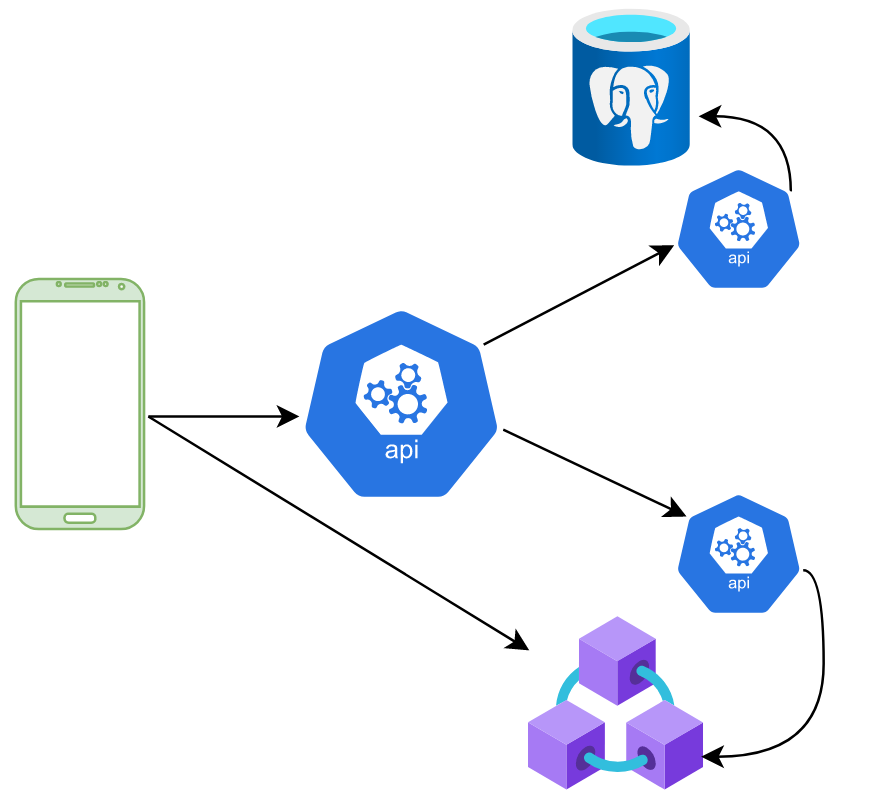
\includegraphics[width=0.6\linewidth]{figs/Desarrollo/Arquitectura}
  \caption[Hash]{Arquitectura de la aplicación Estublock}
  \label{fig:estublockArch}
\end{figure}


\subsubsection{Arquitectura}

\subsubsection{Interaz de Usuario}


% --------------------------------------------------
\subsection{Desarrollo de Microservicio Externo}
% --------------------------------------------------
\subsection{Comunicación con la Red Blockchain}
% --------------------------------------------------
\subsection{A Futuro}



% ##################################################
% ##################################################
\section{SDK}
% --------------------------------------------------
\subsection{Diseño del SDK}
% --------------------------------------------------
\subsection{Como Incorporarlo en Otras Aplicaciones}



% ##################################################
% ##################################################
\section{Documentación}



